\section{Eksperimenti 2. faze}
\subsection{Preliminarni testi}
Z laboratorijskimi eksperimenti v 1. fazi smo dobili zadovoljive rezultate, težave pa so nastale pri uporabi postopka na terenu. Zato smo v 2. fazi optimizirali posamezne segmente elementarnega postopka estimacije fizioloških parametrov. Te smo tudi uporabili v končni preiskavi. V preliminarnih testih so opisani tudi drugi postopki, ki smo jih potrebovali zaradi uporabe Kinect kamer.


\subsubsection{Združevanje slik iz dveh Kinect kamer}\label{sec:zdruzevanje}

\paragraph{Združevanje z značilkami}
Časovno sinhornizirana zaporedja slik smo poskušali združiti z metodo panoramskega šivanja slik z uporabo značilk, kot je opisano v delu \cite{brown2007automatic}. Tu smo namesto SIFT značilk uporabili SURF značilke.


\paragraph{Združevanje s kontrolnimi točkami}
Zaporedja slik smo poskušali združiti z ročnim določevanjem kontrolnih točk.


\paragraph{Prilagojeno združevanje}
Zaradi nezadovoljivih rezultatov klasičnih metod združevanja stereo slik, smo razvili metodo, ki je prilagojena za Kinect kamere. Iz kamer smo pridobili intrinzične parametre infra-redečega (IR) senzora, in sicer: slikovni koordinati goriščne razdalje $f_u$ in $f_v$ ter slikovni koordinati optičnega središča slike (ang. principal point) $c_u$ in $c_v$. Intrinsične parametre smo uporabili za določitev intrizične matrike $\vec{M}_{int}$ po enačbi \eqref{eq:intrinsic}.


Ker pravih ekstrinsičnih parametrov kamer nismo poznali, smo jih le ocenili z metodo določevanja sečišča vidnih polj obeh kamer. Sečišče je prikazano kot rdeča linija na sliki \ref{fig:zdruzevanje}. S to metodo smo določili translacijski vektor $\vec{t} = \left [ t_x~ t_y~ t_z \right]^\top$ in rotacijsko matriko $\vec{R}$ iz Eulerjevih kotov.

S sledenjem igralca z DS-KCF algoritmom, smo s pomočjo projekcijske matrike \eqref{eq:projection-matrix} določili center tarče v metričnih enotah za vsako sliko zaporedja leve in desne kamere. Kadar slikovni element ni vseboval podatkov globine, smo za center tarče izbrali najbližji slikovni element z veljavno globino.

Prva slika združenega zaporedja je bila slika kamere, kjer se igralec prvič pojavi. Nadaljne slike smo izbirali med zaporedjema kamer glede na pozicijo centra tarče. Ko je šel center tarče skozi upragovljeno mejo, ki je na sliki \ref{fig:zdruzevanje} prikazana z modro linijo smo preklopili na drugo kamero. Razdalja med pragom in sečiščem je znašala \SI{200}{mm}.


\begin{figure}[htb]
	\centering
	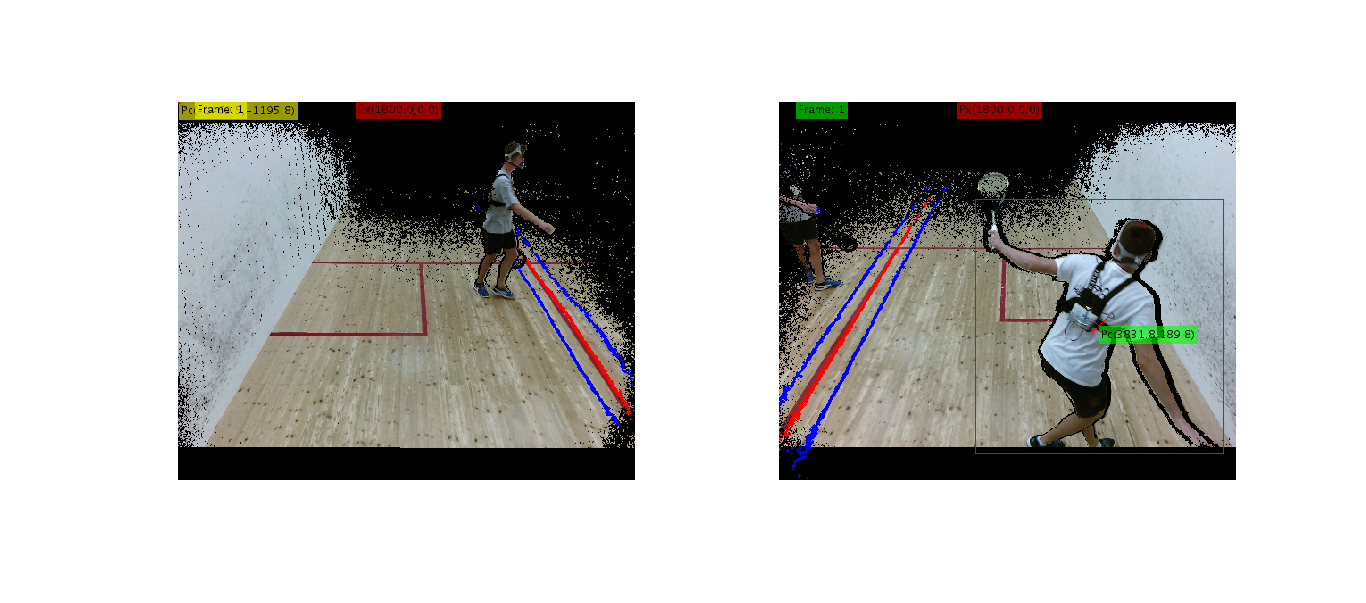
\includegraphics[width=\columnwidth]{./Slike/zdruzevanje-example.png}
	\caption[Določevanje sečišča vidnih polj leve in desne Kinect kamere]{Določevanje sečišča vidnih polj leve in desne Kinect kamere. Na sliki sta prikazani prvi sliki zaporedja leve in desne Kinect kamere 1. seta 2. igre terenskega eksperimenta iz 2. faze. Označen je 4. igralec. Zelena barva koordiat središča tarče predstavlja izbrano kamero. Kamera z rumeno barvo ni izbrana. Sečišče je rdeča linija. Modri liniji sta pragova za preklop med kamerama. Ležita \SI{200}{mm} levo in desno od sečišča.}
	\label{fig:zdruzevanje}
\end{figure}



\subsubsection{Mrežno iskanje \texorpdfstring{$\nu$}{nu}-RBF}
Med evaluacijo eksperimentov 1. faze smo ugotovili, da z regresijo \esvr pogosto dobimo preobremenjene (ang. Overfitted) modele. Pri takih modeli je število podpornih vektorjev zelo visoko. Lahko se zgodi, da postanejo vsi vektorji značilk podporni vektorji. Preobremenjeni modeli lahko sicer dajejo solidne rezultate, vendar pa so ti nerealistični. Takoj, ko bi v tak model vnesli rahlo spremenjene podatke, ne bi več delovali.

Zaradi tovrstnih problemov smo v našem postopku regresijo \esvr zamenjali z \nusvr. Izkazalo se je, da tudi ta ne deluje, čeprav pri njej uporabljamo dodatni parameter $\nu$, s katerim v teoriji kontroliramo razmerje števila podpornih vektorjev, kot je opisano v poglavju \ref{sec:regresija-nusvr}. Chang et. al nam v delu \cite{chang2002training} parameter $\nu$ bolj natačno opiše kot spodnjo mejo razmerja števila podpornih vektorjev. Parameter $\nu$ tako v resnici ne predstavlja omejitve, s katero bi kaznovali prekomerno učneje modela. V ta namen smo razvili mrežno iskanje \nurbf, ki je predstavljeno v poglavju \ref{sec:nurbf}. 

Razvito mrežno iskanje \nurbf uporablja regresijo \nusvr in jedro RBF, zato smo ju uporabljali tudi za učenje modelov. Celoten postopek zato krajše imenujemo kar \nurbf.

\paragraph{Optimizacija parametrov}
Najprej smo optimizirali parameter $\numax$. Za tovrstno optimizacijo smo ponovno naučili \textit{mixed} modele iz 1. faze, pri čemer smo za mrežno iskanje uporabili nov postopek. Modele smo nato uporabili za testiranje na učnih podatkih terenskih eksperimentov 1. faze. S takim postopkom smo izluščili slabe \textit{squash} modele, ki bi oteževali pravilno evaluacijo rezultatov pri optimizaciji.

Za optimizacijo smo uporabili HOOF-HAFA deskriptor in naslednje vrednosti parametrov: začetna vrednost $\nu$ $0.1$ in standardni odklon za Gaussov filter $\sigma=5$. Za $\numax$ smo uporabili 400, 800 in 1200 podpornih vektorjev. 

Z optimiziranim parametrom $\numax$ smo \nurbf preizkusili še na elementarnih modelih. Tu smo za razliko od eksperimentov iz 1. faze poleg \nurbf uporabili razširjeni HOOF-HAFA deskriptor.







\subsubsection{Jedro GHI}
Kot smo že opisali v poglavju \ref{sec:ghi}, je jedro GHI primerno za histogramske deskriptorje. To jedro smo preizkusili zaradi problemov postopka iz 1. faze, kjer smo uporabili RBF jedro. GHI smo implementirali z \nurbf, s to razliko, da predikcij križnih validacij nismo filtrirali. S tem smo zagotovili, da se ta postopek od tistega iz 1. faze razlikuje le v uporabi drugega jedra in parametra $\numax$. Zaradi slednjega smo zagotovili, da se modeli niso prenaučili. V nasprotnem primeru, bi preobremenjeni modeli oteževali evaluacijo.

GHI smo preizkusili na elementarnih modelih, z HOOF deskriptorjem. Rezultate smo filtrirali s Kalmanovim filtrom. Pri uporabi GHI jedra smo značilke skalirali na intervalu $[0,~1]$ zaradi hitrejšega učenja. Parameter $\numax$ je znašal \SI{50}{\%} podpornih vektorjev. 






\subsubsection{Optimizacija Gaussovega filtra}
Pri optimizaciji Gaussovega filtra smo določili optimalni standardni odklon $\sigma$ z uporabo dveh metrik, in sicer: koren srednje kvadratične napake (RMSE) in razmerje med signalom in šumom (SNR). Pri RMSE metriki smo določili napako med učnimi vzorci in njihovo predikcijo. Pri SNR metriki smo za signal uporabili referenčne učne vzorce. Za šum smo uporabili rezidualni ali preostali šum. Tega smo dobili z odštevanjem filtriranih vzorcev od referenčnih. SNR metrika tako določa uspešnost izločevanja šuma, RMSE metrika pa pravilnost določevanja kateri podatki spadajo v signal in kateri v šum.


Teste smo izvajali na vseh eksperimentih 1. sklopa, pri čemer smo uporabili \nurbf mrežno iskanje s \SI{50}{\%} podpornih vektorjev. Za filtriranje pri mrežnem iskanju smo izbrali najmanjši filter s $\sigma = 1$. Testirali smo naslednje standardne odklone Gaussovega filtra: $1, 3, 5, 11, 21, 31$ in $51$. 




\subsubsection{Normalizacija HAFA deskriptorjev}
V praksi se pokaže, da prvotni HAFA histogram ne deluje zadovoljivo, saj se histogram lahko močno spreminja pri uporabi sledilnika. Zaradi neidelanega delovanja sledilnika področje tarče skozi čas spreminja svojo velikost, to pa vpliva na vrednosti stolpcev HAFA histograma. Ker te dobimo s preštevanjem slikovnih elementov z enako amplitudo hitrosti bo manjše področje posledično zmanjšalo celoten histogram. Pri HOOF histogramih tega problema praktično nimamo, saj ima majhen vpliv. Razlog tiči v računanju vrednosti stolpcev HOOF histograma. Njihove vrednosti dobimo s seštevanjem amplitud in ne njihovim preštevanjem. Te so zato pred normiranjem praviloma večje.

Probleme sledilnika smo poskušali kompenzirati z uvedbo amplitudnega faktorja $f_A$. Amplitudni faktor je pravzaprav razmerje med velikostjo področja igralca na terenskih testih in velikostjo merjenca na tekalni stezi. Razmerje lahko preprosto dobimo z razmerjem diagonal področij po enačbi \eqref{eq:diag}, kjer so $w_l$ in $h_l$ širina in dolžina področja na tekalni stezi ter $w_s$ in $h_s$ širina in dolžina področja na terenskih testih.

\begin{equation}
f_A = \frac{\sqrt{w_l^2 + h_l^2}}{\sqrt{w_s^2 + h_s^2}}
\label{eq:diag}
\end{equation}

Velikost diagonale na laboratorijskih testih uporabljamo kot referenco. To pa zato, ker je na teh posnetkih stabilna, saj se le malo spreminja. Koncept amplitudnega faktorja smo preizkusili na enakem postopku, kot pri optimizaciji parametra mrežnega iskanja \nurbf. S takim postopkom smo izluščili slabe \textit{squash} modele, ki bi oteževali pravilno evaluacijo rezultatov pri optimizaciji. Naučili smo modele \textit{diag}, kjer smo uporabili amplitudni faktor in referenčne modele \textit{normal} brez uporabe faktorja za primerjavo. Diagonalo na tekalni stezi smo določili po sliki \ref{fig:diag-bbox}, kjer smo za zgornji levi kot $P_0$ in spodnji desni kot $P_1$ izbrali vrednosti v tabeli \ref{tab:diag}. 


\begin{figure}[htb]
	\centering
	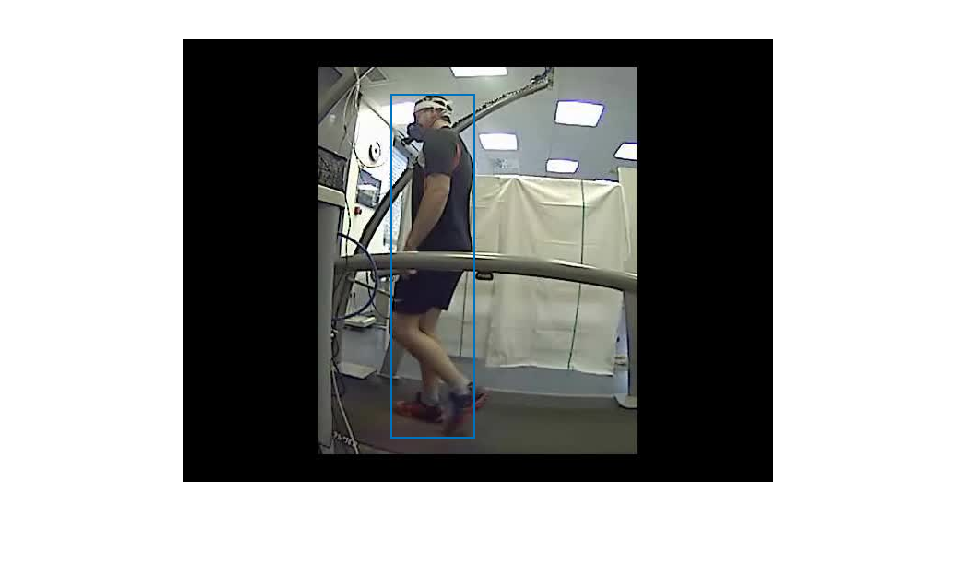
\includegraphics[width=0.6\columnwidth]{./Slike/diag-bbox.png}
	\caption{}
	\label{fig:diag-bbox}
\end{figure}

\begin{table}[htb]
	\centering
	\begin{tabular}{l S[table-format=3] S[table-format=3]}
		\toprule
		\textbf{Točka} & \thead{$\mathbf{x}$} & \thead{$\mathbf{y}$} \\ 
		\midrule
		$P_0$ & 297 & 82 \\
		$P_1$ & 389 & 452 \\
		\bottomrule
	\end{tabular}
	\caption[Optimalni parameteri RBF jedra modelov za izbiro deskriptorjev]{Optimalni parametri RBF jedra za modele z različnim deskriptorjem.}
	\label{tab:diag}
\end{table}

Pri testiranju smo uporabili parameter $\numax$ \SI{50}{\%} podpornih vektorjev. Za Gaussov filter smo uporabili $\sigma=5$. Značilke smo skalirani na intervalu $[0,~1]$. Za modele z diagonalo smo uporabili parameter $f_{A}=381.266$. Pri učenju smo uporabili optimalne vrednosti parametrov, ki so prikazane v tabeli \ref{tab:diag}. Za evaluacijo rezultatov smo uporabili predikcije testnih vzorcev z modeli s zakasnitvijo.



\begin{table}[htb]
	\centering
	\begin{tabular}{l S[table-format=3] S[table-format=1.3] S[table-format=1.1] S[table-format=1.3]}
		\toprule
		\textbf{Model} & \thead{$\mathbf{C}$} & \thead{$\mathbf{\gamma}$} & \thead{$\mathbf{\nu}$} & \thead{MSE} \\ 
		\midrule
		NORMAL & 256 & 0.354 & 0.1 & 5.297 \\
		DIAG & 256 & 0.354 & 0.1 & 5.297 \\
		\bottomrule
	\end{tabular}
	\caption[Optimalni parameteri RBF jedra modelov za izbiro deskriptorjev]{Optimalni parametri RBF jedra za modele z različnim deskriptorjem.}
	\label{tab:izbira-param-diag}
\end{table}


\subsection{Laboratorijski eksperimenti}
Merjenci so opravili obremenilni test po protokolu Nowatzky. To je stopnjevani test na tekoči preprogi za merjenje maksimalne porabe kisika in oceno aerobne kapacitete posameznika. Test smo izvajali s pomočjo sistema za direktno ergospirometrijo tipa ``breath  by breath'' Cosmed K4B2. Uporabili smo  tekočo  preprogo HP Cosmos.

\subsubsection{Pridobivanje podatkov}
Tekalno stezo smo snemali iz dveh različnih zornih kotov: hrbtni del in stranski del.  Primer hrbtnega in stranskega posnetka je prikazan na sliki \ref{fig:primer-posnetka-stage2}.

\begin{figure}[htb]
	\centering
	\begin{subfigure}{0.45\columnwidth}
		%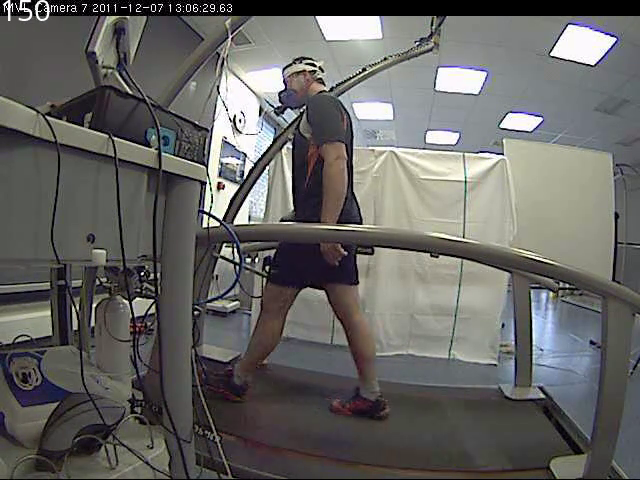
\includegraphics[width=\columnwidth]{./Slike/normal-sv-150.png}
		\caption{stranska slika}
	\end{subfigure}
	~
	\begin{subfigure}{0.45\columnwidth}
		%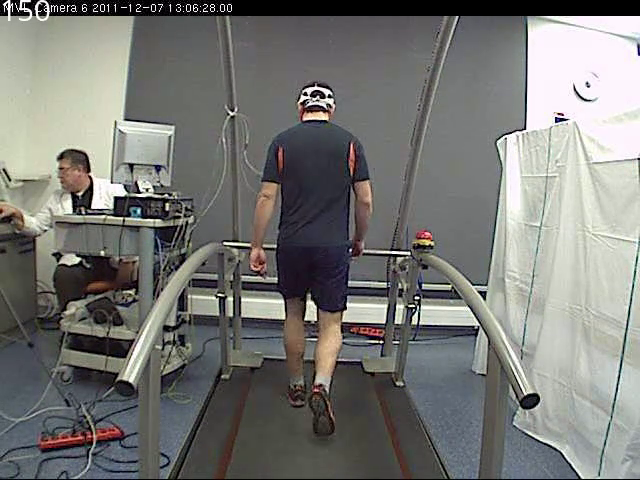
\includegraphics[width=\columnwidth]{./Slike/normal-bv-150.png}
		\caption{hrbtna slika}
	\end{subfigure}
	\caption{Hrbtna in stranska 150. slika RGB posnetkov iz prve serije.}
	\label{fig:primer-posnetka-stage2}
\end{figure}

Snemali smo z dvema Microsoft Xbox Kinect V2 kamerama. Pridobili smo barvne RGB in globinske DEPTH slike. Snemali smo v ločljivosti $512 \times 424$. Hitrost posnetkov je znašala \SI{30}{fps}. Kameri smo časovno sinhronizirali po NTP protokolu.

\subsubsection{Protokol izvajanja meritev}
Test smo pričeli s tri minutnim ogrevanjem s hitrostjo teka \SI{5}{\km\per\hour}, pri naklonu preproge \SI{0}{\%}. Nadaljevali smo s 3 minutnim tekom s hitrostjo \SI{6}{\km\per\hour}. Po treh minutah smo naklon tekoče preproge  dvignili za \SI{2}{\%} in ga nismo več spreminjali. Po pretečeni minuti na  tretji stopnji (hitrost \SI{6}{\km\per\hour}, naklon \SI{2}{\%}) se je hitrost teka vsaki dve  minuti  povečevala za \SI{1}{\km\per\hour}. Test smo izvajali brez prekinitve do pojava objektivnih oz. subjektivnih razlogov za prekinitev testa. Po koncu testiranja je sledilo še \SI{5}{min} hoje pri  hitrosti \SI{2}{\km\per\hour} ter \SI{0}{\%} naklonu.  

\subsubsection{Protokoli postopka procesiranja}
!!!!!!!!!!!!!
Interpolacija podatkov
Kot smo že omenili so bile meritve fizioloških parametrov izvedene z vzorčenjem \SI{5}{\s} oziroma s frekvenco \SI{0.2}{\hertz}. Hitrost posnetkov je bila \SI{30}{fps} za RGB in \SI{25}{fps} za IR slike. Zaradi neskladja frekvenc vzorčenja slik in fizioloških parametrov, smo te interpolirali s pomočjo Matlabove funkcije \texttt{interp1}.

Za izbrano področje slike iz zaporedja posameznega posnetka smo nato izračunali optični tok. Primer dobljenega optičnega toka je prikazan na sliki \ref{fig:opticni-tok-stage1}.

Sledilo je generiranje HOOF deskriptorjev, ki smo jih pred tem optimizirali po postopku, opisanem v poglavju \ref{sec:optimizacija-hoof}. Za parameter smo izbrali $N_{HOOF} = 60 $, ker je dal najbolj optimalne rezultate. Primer HOOF deskriptorjev lahko vidimo na sliki \ref{fig:hoof-znacilke}.

Modele smo učili z metodo podpornih vektorjev $\epsilon$-SVR in jedrom RBF. Regresijske parametre jedra smo optimizirali z metodo mrežnega iskanja. Naučili smo \num{8} elementarnih modelov, ki smo jih razdelili na dve kategoriji: na \textit{hr} modele, ki predvidevajo srčni utrip in modele \textit{eem}, ki predvidevajo porabo energije v \si{\kcal\per\min}. Kategoriji sta nadalje razdeljeni glede na zorni kot kamere: \textit{sv} modeli za stransko kamero in \textit{bv} modeli za hrbtno kamero. Eksperimente smo razširili z vpeljavo zakasnitve med referenčnim fiziološkim parametrom in merjenim parametrom iz slik posnetka. Z eksperimenti, ki so označeni z \textit{lag} kratico, smo preverili predlagano časovno zakasnitev med vzbujanjem in fiziološkim odzivom. 

Generirali smo tudi dodatne modele, in sicer: \textit{crop} modele, \textit{mixed} modele, \textit{track} modele, kjer smo uporabili sledilnik in obremenitvene modele. Ti so deljeni na \textit{scale} modele in \textit{proj} modele.

Vse tipe eksperimentov smo križno testirali glede na enak tip eksperimenta, le z drugim zornim kotom kamere. Uporabljen zorni kot kamere za križno testiranje je v imenih modelov zapisan v oklepajih. Rezultate smo pred testiranjem filtrirali s Kalmanovim filtrom. Uporabljeni parametri so opisani v poglavju \ref{sec:implementacija-kalman}.






snemanje s kinektom sledenje s DS-KCF uporaba diagonale   HOOF-HAFA deskriptor Prostoski tok PD-FLOW  \nurbf (\nusvr RBF jedro) Gaussovo filtriranje.

1. Za testiranje vsak 3ji frame, za treniranje pa vse ostalo. Povprečenje vseh 6 setov. (Neodvisnost od časovnega povečevanja porabe) 

2. Za trening prvih 70 \% vzorcev za test ostalih 30 \%. Povprečenje vseh 6 setov. (Za prikaz odvisnosti od časovnega povečanja porabe) 

3. Protokol 1 pri čemer treniram na 4 igralcih in testiram na ostalih 2 ter povprečim rezultata. (Prikaz delovanja za različne igralce)

\subsubsection{Določitev zakasnitve fiziološkega odziva}
!!!!!!!!!!!!!!!!!!

\begin{figure}[!htbp]
	\centering
	\begin{subfigure}[t]{0.45\columnwidth}
		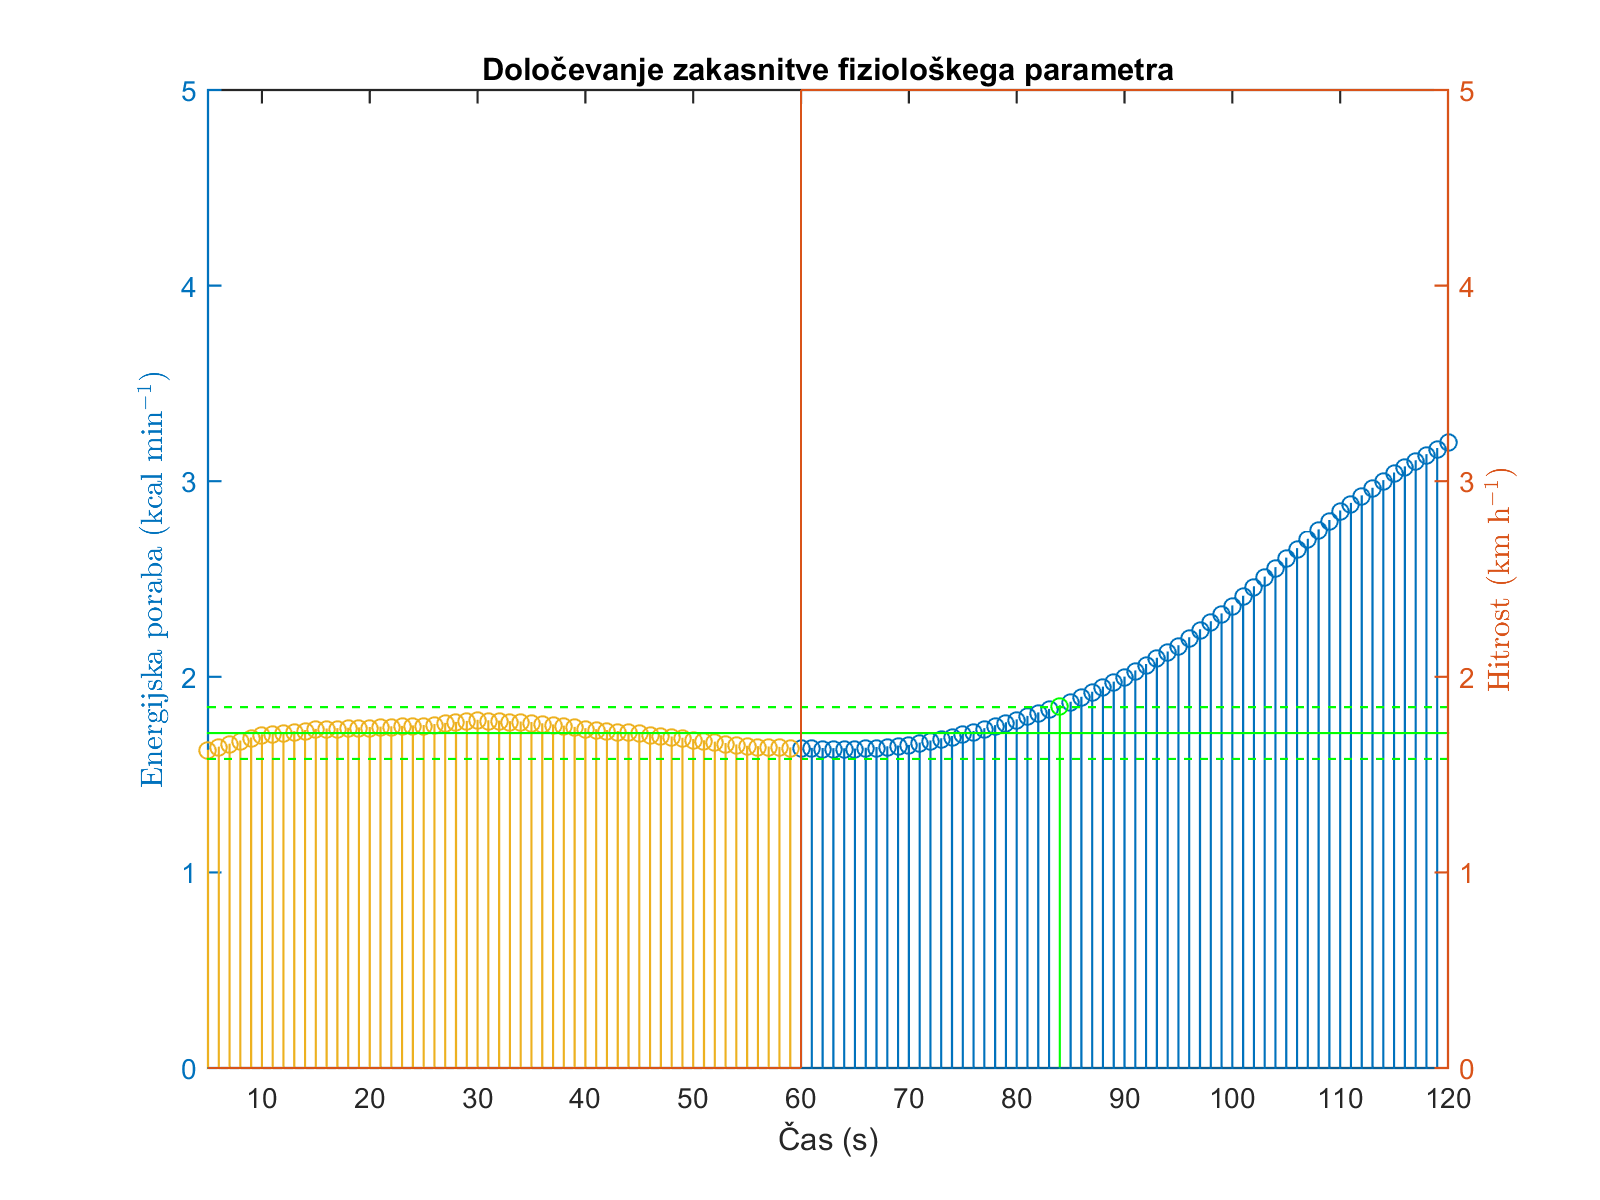
\includegraphics[width=\columnwidth]{./Slike/lag-estimation-1-eem.png}
		\caption{Zakasnitev za subjekt 1.}
		\label{fig:lag-estimation-1-eem}
	\end{subfigure}
	~
	\begin{subfigure}[t]{0.45\columnwidth}
		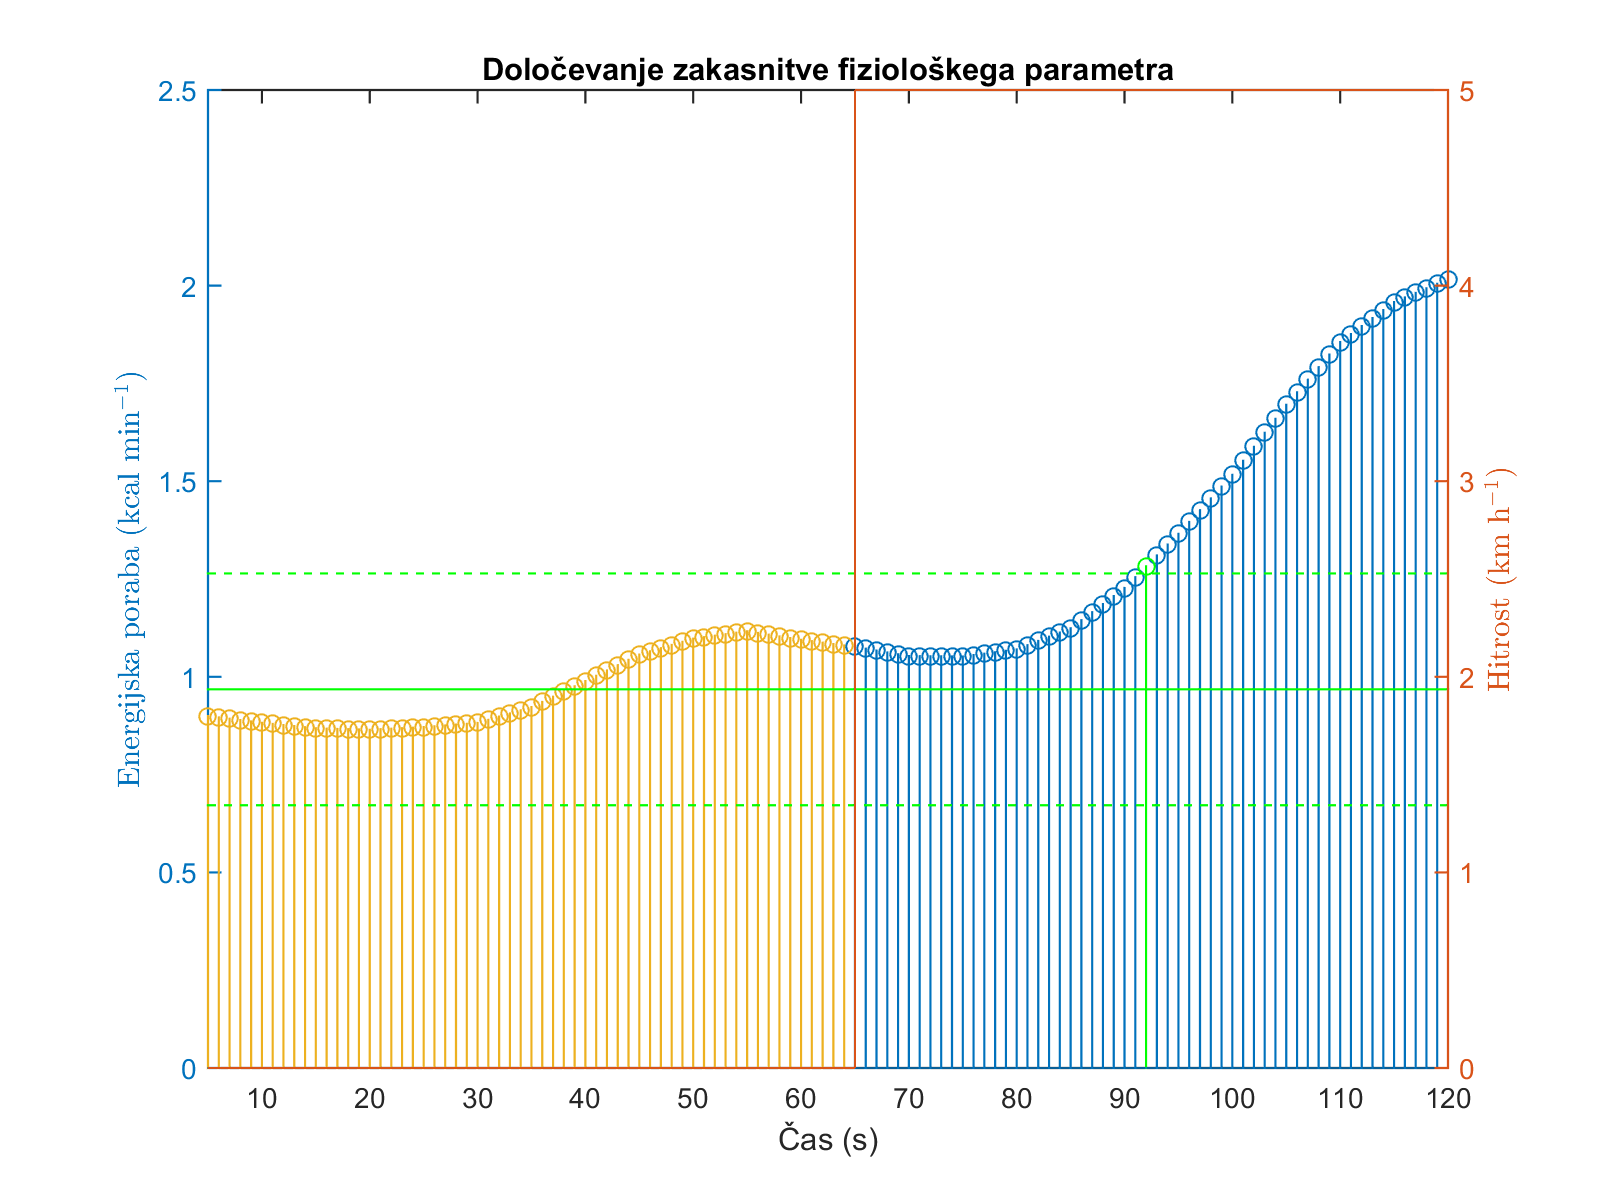
\includegraphics[width=\columnwidth]{./Slike/lag-estimation-2-eem.png}
		\caption{Zakasnitev za subjekt 2.}
		\label{fig:lag-estimation-2-eem}
	\end{subfigure}
	~
	\begin{subfigure}[t]{0.45\columnwidth}
		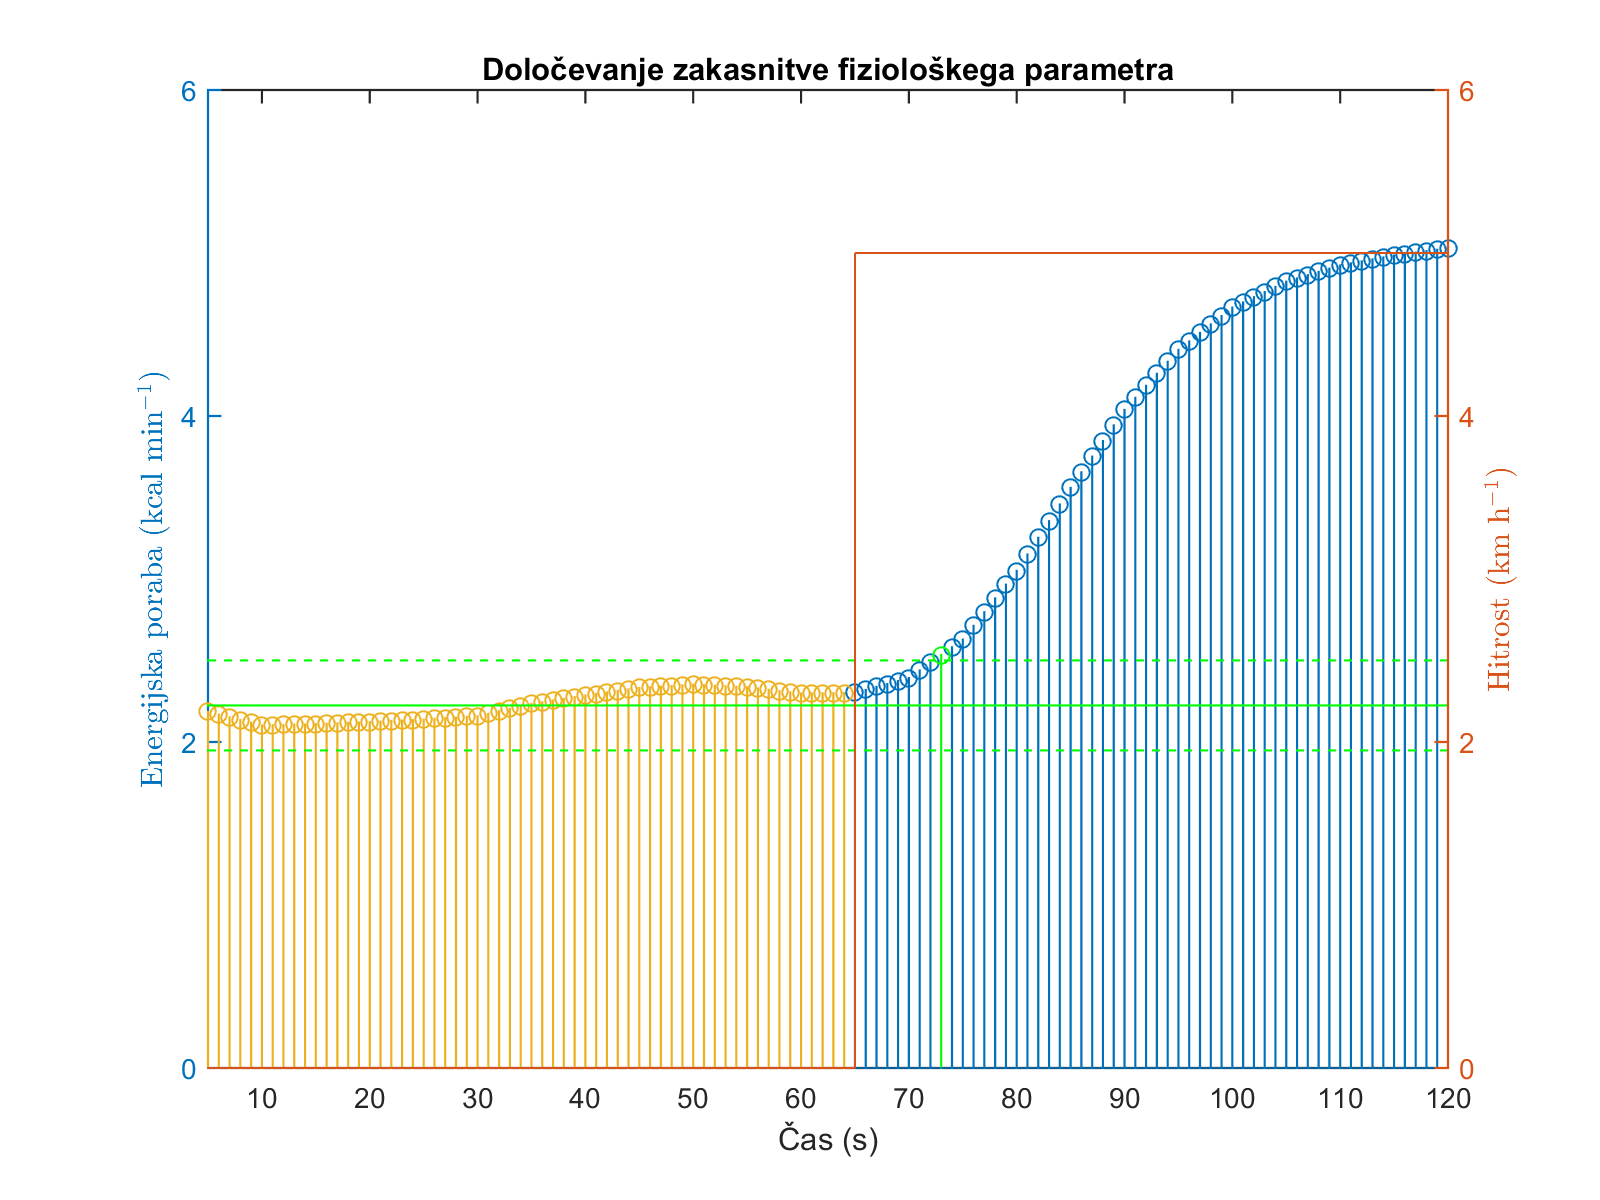
\includegraphics[width=\columnwidth]{./Slike/lag-estimation-3-eem.png}
		\caption{Zakasnitev za subjekt 3.}
		\label{fig:lag-estimation-3-eem}
	\end{subfigure}
	~
	\begin{subfigure}[t]{0.45\columnwidth}
		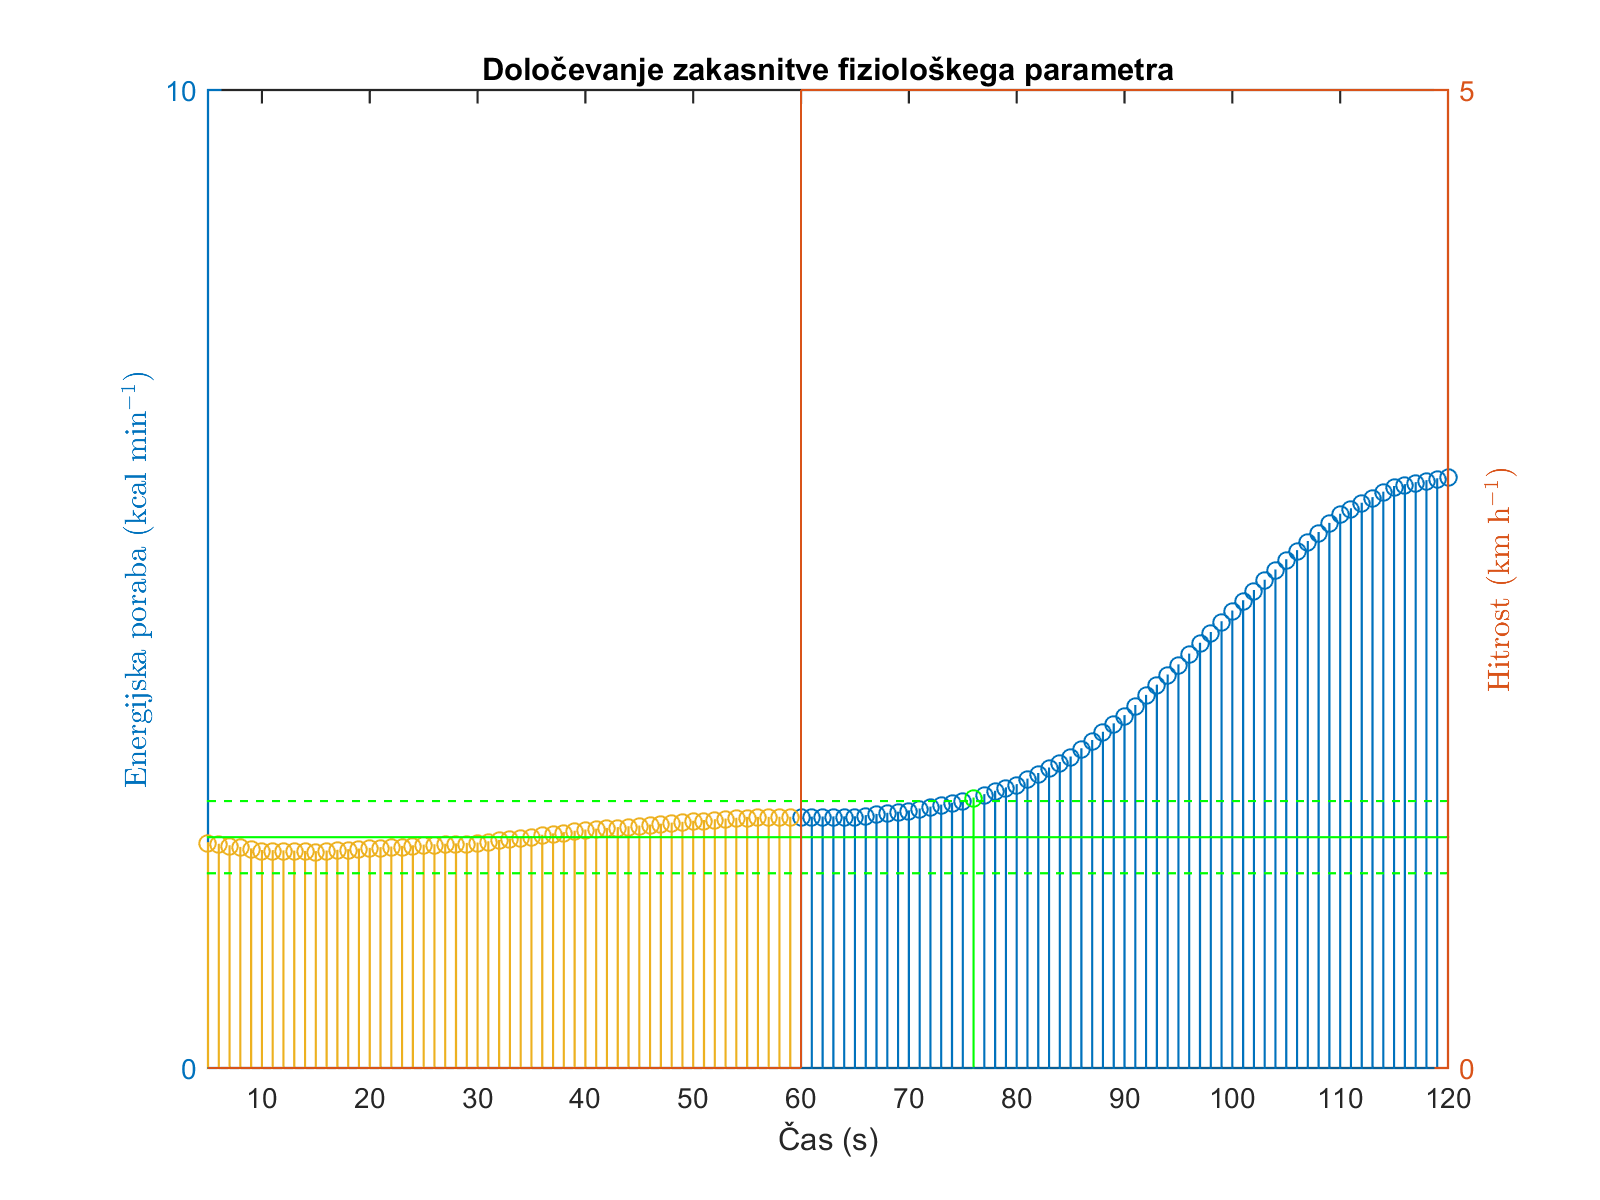
\includegraphics[width=\columnwidth]{./Slike/lag-estimation-4-eem.png}
		\caption{Zakasnitev za subjekt 4.}
		\label{fig:lag-estimation-4-eem}
	\end{subfigure}
	~
	\begin{subfigure}[t]{0.45\columnwidth}
		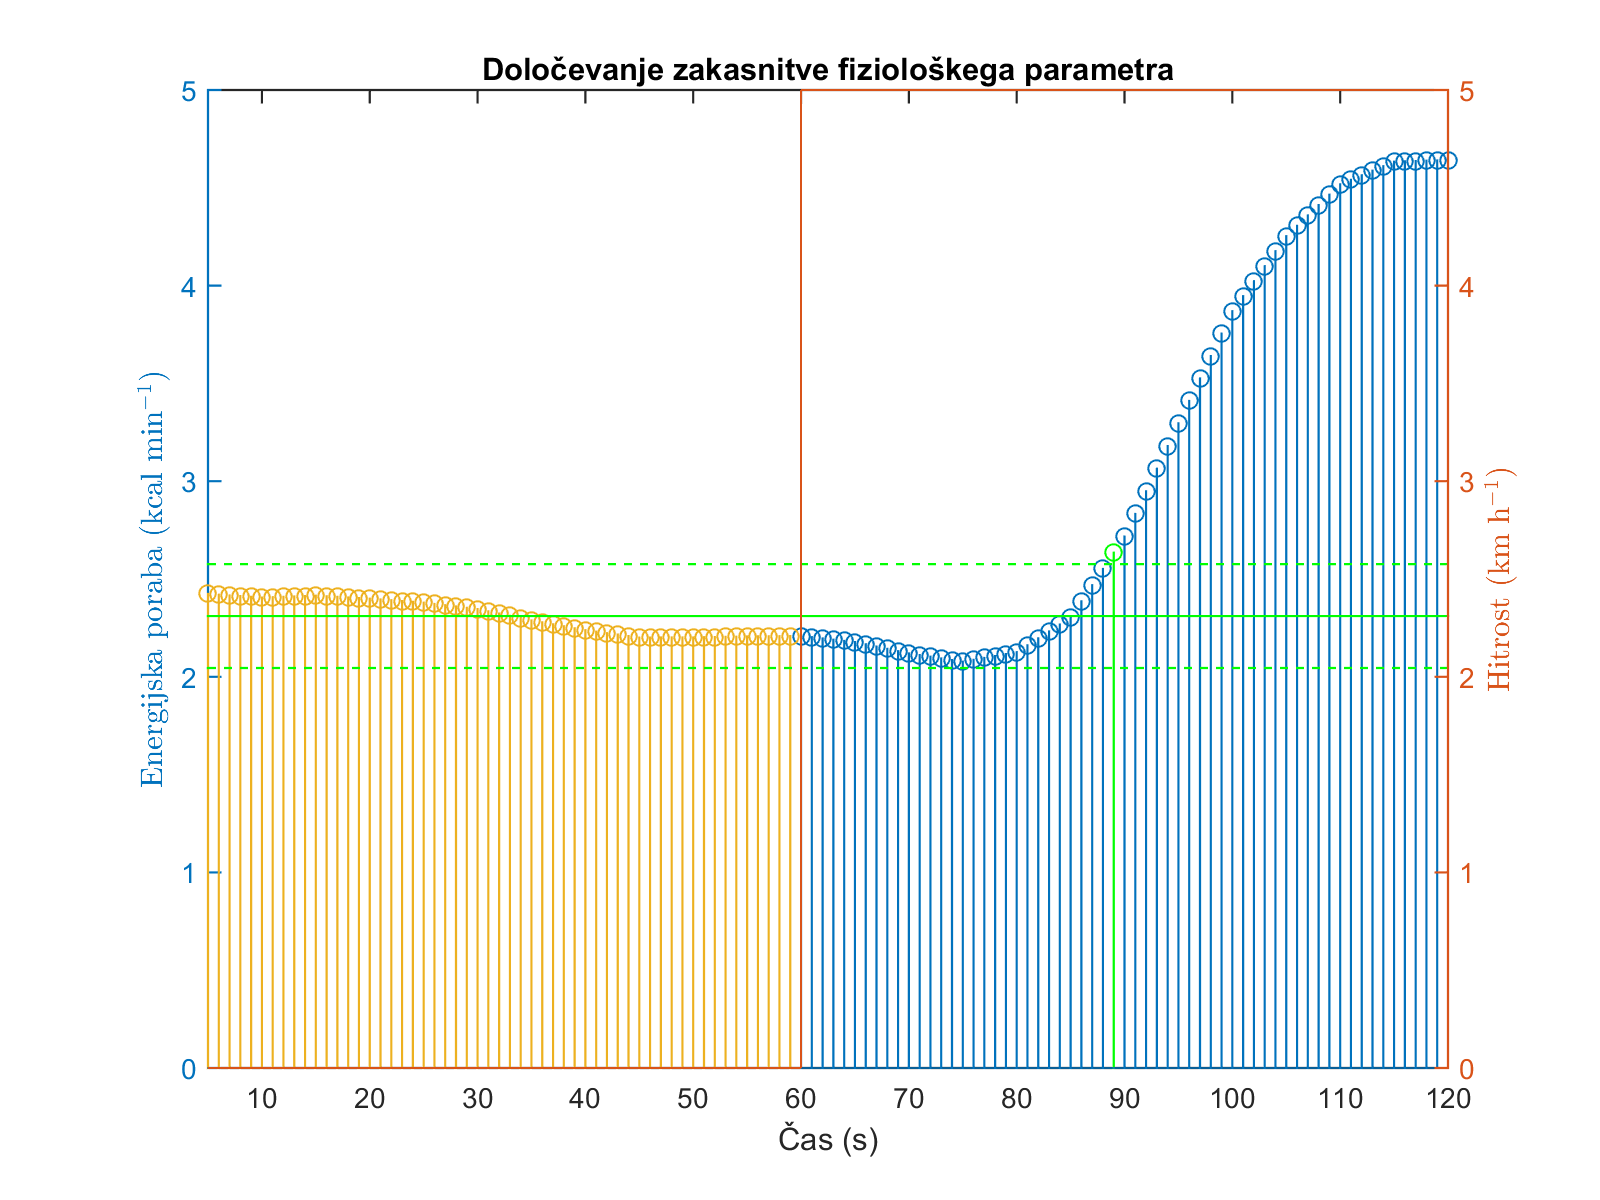
\includegraphics[width=\columnwidth]{./Slike/lag-estimation-5-eem.png}
		\caption{Zakasnitev za subjekt 5.}
		\label{fig:lag-estimation-5-eem}
	\end{subfigure}
	~
	\begin{subfigure}[t]{0.45\columnwidth}
		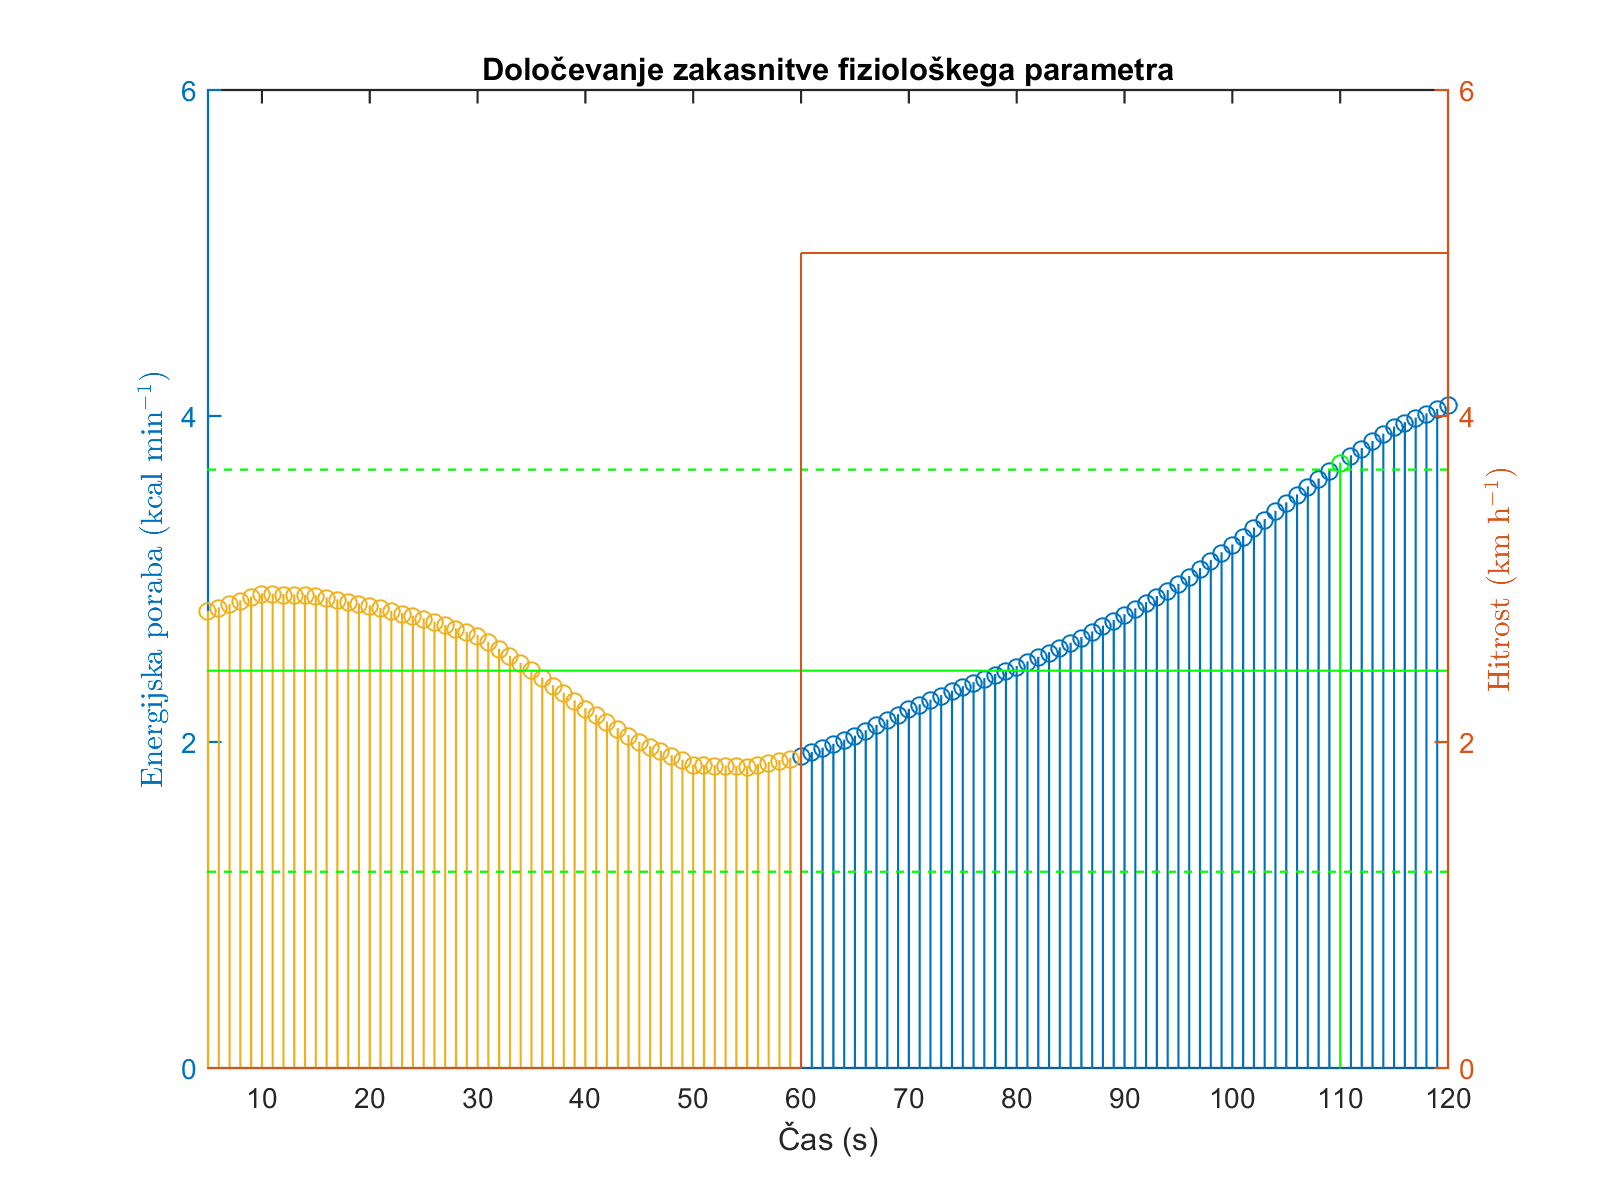
\includegraphics[width=\columnwidth]{./Slike/lag-estimation-6-eem.png}
		\caption{Zakasnitev za subjekt 6.}
		\label{fig:lag-estimation-6-eem}
	\end{subfigure}
	\caption{}
	\label{fig:lag-estimation-stage2}
\end{figure}










\subsection{Terenski eksperimenti}

Kaj smo delali?

Kako smo snemali?

\begin{figure}[htb]
	\centering
	\begin{subfigure}{0.45\columnwidth}
		%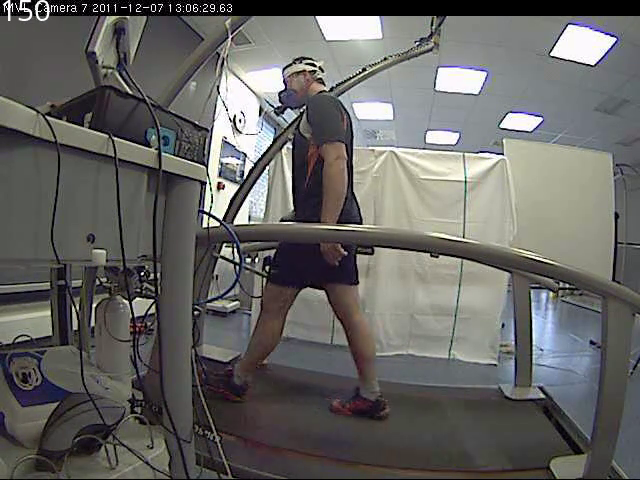
\includegraphics[width=\columnwidth]{./Slike/normal-sv-150.png}
		\caption{stranska slika}
	\end{subfigure}
	~
	\begin{subfigure}{0.45\columnwidth}
		%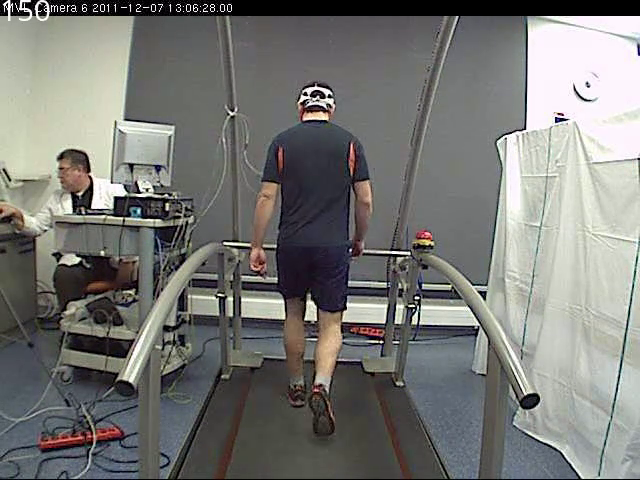
\includegraphics[width=\columnwidth]{./Slike/normal-bv-150.png}
		\caption{hrbtna slika}
	\end{subfigure}
	\caption{Hrbtna in stranska 150. slika RGB posnetkov iz prve serije.}
	\label{fig:primer-posnetka-teren}
\end{figure}

Kakšno opremo smo uporabili?

Snemali smo z dvema Microsoft Xbox Kinect V2 kamerama. Pridobili smo barvne RGB in globinske DEPTH slike. Snemali smo v ločljivosti $512 \times 424$. Hitrost posnetkov je znašala \SI{30}{fps}. Kameri smo časovno sinhronizirali po NTP protokolu.

Kakšen je protokol testiranja?

